\section{Characterization Problem Results}
\label{sec:CharResults}

To quantify the $\Omega$-method success for a variety of anisotropy-inducing
physics, we will present various forms of the Figure of Merit, as described in
Section \ref{sec:successmetrics}.
In the preceding subsections, a
subset of flux anisotropy-inducing physics have been identified
and a subset of problems that contain these physics have been conceived.
In this section, the results for CADIS-$\Omega$, CADIS, and nonbiased Monte Carlo
will be presented for each of these problems. Explanations on the performance of
the $\Omega$ methods will accompany the results for each problem. In some cases,
variants of problems were run to confirm or refute observations seen
in other problems.

\subsection{Computational Specifications}
\label{subsec:comp_specs}

As noted in a number of the previous sections, hybrid methods require both a
deterministic and a Monte Carlo calculation to obtain a problem result. These
transport codes require different computational parameters to obtain an answer.
For the characterization problems the computational parameters are summarized in
Table \ref{tab:simulation_defaults}; the parameters for the deterministic and
Monte Carlo calculations are demarcated in the table.

\begin{table}[h!]
  \centering
  \begin{tabular}{l|m{5cm}}
\toprule
Parameter Type & Parameter Value \\
\midrule \midrule
\multicolumn{2}{c}{ADVANTG Values$^1$} \\
\midrule
P$_N$ Order               &    $3$ \\
Quadrature Type           &  Quadruple Range \\
Quadrature Order          &    $10$ \\
Spatial Solver            &  Step Characteristic \\
Energy Group Library$^{\dagger}$     &    27G19N \\
Boundary Conditions & vacuum \\
\midrule \midrule
\multicolumn{2}{c}{MCNP Values$^2$} \\
\midrule
Particle Count      &   $1e7$ \\
Boundary Conditions & vacuum \\
\bottomrule
\end{tabular}
\begin{flushleft}
\footnotesize{
  $^1$ ADVANTG runs of the characterization problems
  were run on 16 cores of a 32 core node, with 256Gb of memory on
  an Oak Ridge National Laboratory compute cluster maintained by the Radiation
  Transport and Nuclear Systems Division. \\
  $^2$ MCNP runs of the characterization problems were run on the same
 machine, with 256Gb of memory but using all 32 cores of the node. \\
  $^{\dagger}$ Parameter type that has no default in ADVANTG.}
\end{flushleft}


  \caption[Default simulation values for characterization problems.]{
    Default simulation values for the characterization problems. The values for
    ADVANTG primarily signify parameters used to run Denovo, with exceptions for
    calculating biasing parameters, which is done exclusively in ADVANTG.
    MCNP-specific values are those used for Monte Carlo runs.
  }
  \label{tab:simulation_defaults}
\end{table}

The first portion of the table summarizes the values used by ADVANTG. Note that
these values all pertain to the Denovo deterministic solver, which is set up by
ADVANTG. The parameter types marked with an asterisk have no default in ADVANTG.
We have chosen to use a relatively course 27 group energy group library.
Because the characterization problems are meant to identify the method's
performance pertaining to flux anisotropy, and we expect the energy group
structure to have little effect on anisotropy conditions, we opted for a
computationally inexpensive energy group mesh for the deterministic solver.
The values without an asterisk are ADVANTG default values.
They are also good choices for
initial characterization of the method. This is because a novice user may opt to
use these parameters for an initial solution on a problem for which they may have
little intuition. Further, these values are defaults in ADVANTG for their
computational stability--such as not having negative valued weights or fluxes,
stable convergence, a relatively fast time to a solution, etc.--so they should
be good initial parameters with which to study the characterization problems.

The latter section of the table summarizes the Monte Carlo code MCNP values for
each of the problems. The value of $1e7$ particles as a particle cutoff
was chosen because it made the
error bins in the majority of the nonbiased Monte Carlo
characterization problems less than 100\%. In some problems that are
extraordinarily difficult for Monte Carlo to solve without biasing, there were
tally bins with very high errors. In the following subsections they will be
clearly indicated. Time cutoffs were not chosen because
we decided to measure how effective the $\Omega$ methods were at reducing the
variance per particle. Depending on the flux maps generated from CADIS and
CADIS-$\Omega$, the time to transport a finite amount of particles may vary. As
a result, the reported times from a simulation can tell us whether the method
requires more sampling than other methods.

Each problem presented in Section \ref{sec:CharResults} will
use the values specified in Table \ref{tab:simulation_defaults}
unless otherwise noted.
Times to transport the Monte Carlo particle quantity varies between methods
due to differences in sampling. Monte Carlo and ADVANTG
inputs and directions on how to acquire them are
provided in Appendix \ref{sec:github_codes}.

\subsection{Maze Variants}
\label{subsec:resultsmaze}
\subsubsection{Single Turn}
[Table of FOMs for this problem] \\

\begin{table}[h!]
  \centering
  \begin{tabular}{lrrrrr}
\toprule
{} & cadis &             & cadisangle &             & analog \\
{} &    MC & MC\_adjusted &         MC & MC\_adjusted &     MC \\
\midrule
tally avg   &   327 &         248 &        224 &          71 &  0.054 \\
max RE      &  1.46 &        1.11 &       1.02 &       0.322 & 0.0393 \\
min RE      &   113 &        85.6 &         71 &        22.5 &    -- \\
time (mins) &  51.5 &          68 &       35.5 &         112 &   25.5 \\
\bottomrule
\end{tabular}

  \caption[Figure of Merit comparison for single turn maze.]{Figure of Merit
    comparison for single turn maze. The FOMS are
  quantified using three relative error results and two different timing results.
  The relative errors used are the tally average relative error, the tally maximum relative
  error, and the tally minimum relative error; the times are total walltimes for
  the Monte Carlo calculation and the sum of the hybrid method software, the
  deterministic tranport time, and the Monte Carlo calculation time.}
  \label{tab:maze1foms}
\end{table}

[Plot of tally results for this problem] \\

\begin{figure}[h!]
  \centering
  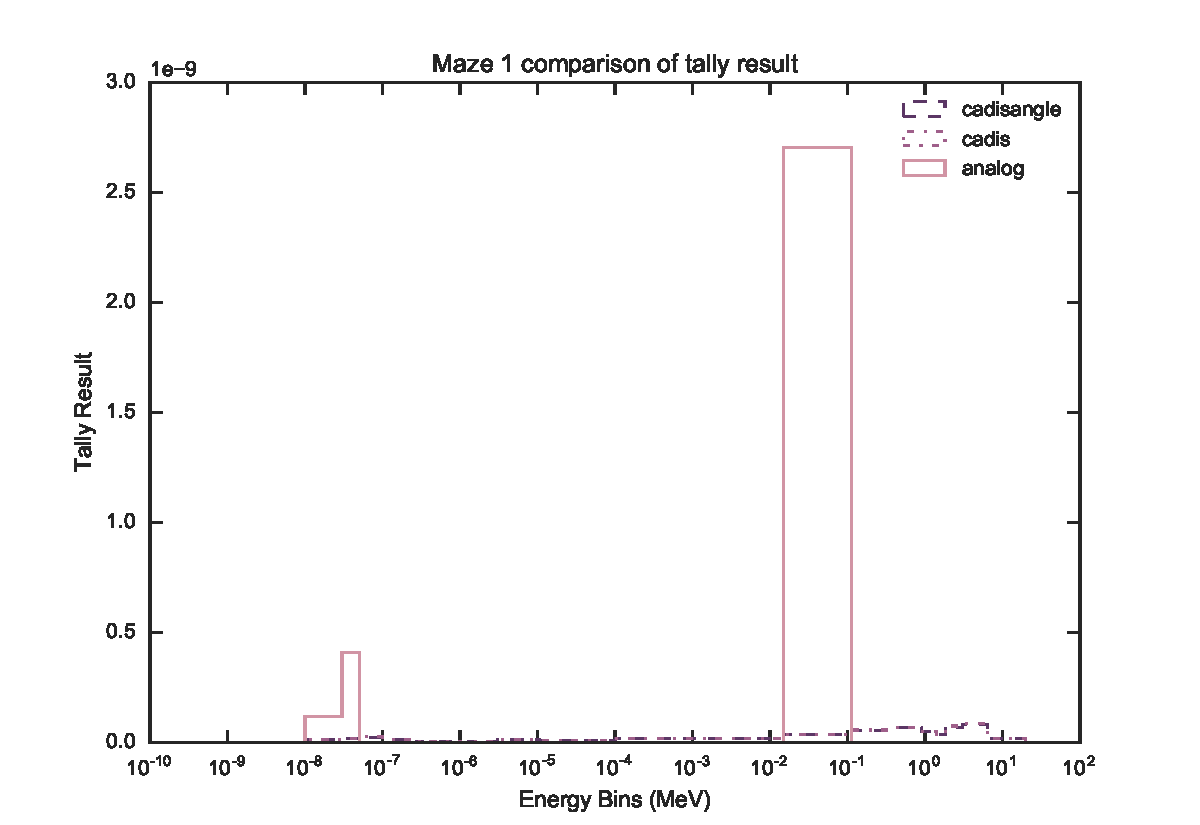
\includegraphics[height=10cm]{./chapters/characterization_probs/figures/maze1/maze_1_tally_result_compare.pdf}
  \caption[Tally results comparison between methods for single turn labyrinth.]
  {Tally results comparison between methods for single turn labyrinth. This is a fun tally result.}
  \label{fig:maze1result}
\end{figure}

\begin{figure}[h!]
  \centering
  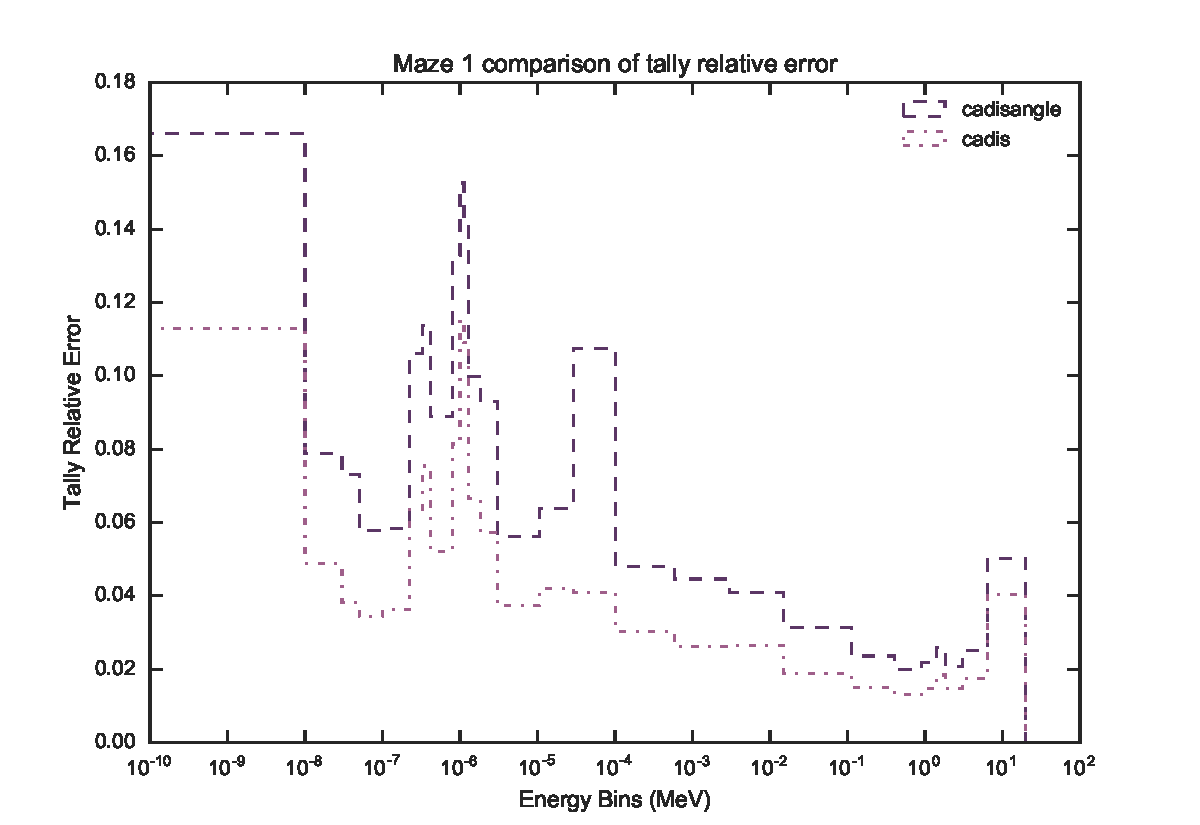
\includegraphics{./chapters/characterization_probs/figures/maze1/maze_1_tally_error_compare.pdf}
  \caption[Tally relative error comparison between methods for single turn
  labyrinth]{Tally relative error comparison between methods for a single turn
  labyrinth. This is a super cool result.}
  \label{fig:maze1result}
\end{figure}
[Plot of anisotropies for this problem] \\

[Summarize results and describe issues affecting performance] \\

\subsubsection{Multiple Turn}
[Table of FOMs for this problem]\\

[Plot of tally results for this problem]\\

[Plot of anisotropies for this problem] \\

[Summarize results and describe issues affecting performance] \\

\subsection{Steel Beam}
\label{subsec:resultbeam}
[Table of FOMs for this problem] \\

[Plot of tally results for this problem] \\

[Plot of anisotropies for this problem] \\

[Summarize results and describe issues affecting performance] \\

\subsection{U-Shaped Corridor}
\label{subsec:resultsucorridor}
[Table of FOMs for this problem] \\

[Plot of tally results for this problem] \\

[Plot of anisotropies for this problem] \\

[Summarize results and describe issues affecting performance] \\

\subsection{Shielding with Rebar}
\label{subsec:resultrebar}
[Table of FOMs for this problem] \\

[Plot of tally results for this problem] \\

[Plot of anisotropies for this problem] \\

[Summarize results and describe issues affecting performance] \\

\subsection{Beam Problem}
\label{subsec:resultsbeam}
[Table of FOMs for this problem] \\

[Plot of tally results for this problem] \\

[Plot of anisotropies for this problem] \\

[Summarize results and describe issues affecting performance] \\

\subsection{Therapy Room}
\label{subsec:resultstherapy}
[Table of FOMs for this problem] \\

[Plot of tally results for this problem] \\

[Plot of anisotropies for this problem] \\

[Summarize results and describe issues affecting performance] \\

